\part{Step Counter Algorithm}

    \chapter{Overview}

        This section shall cover the development and workings of the step counter algorithm. The algorithm aims to extract incidences of steps from the raw accelerometer data from a mobile phone. An example of raw accelerometer data of walking is shown below in Figure \ref{img_accel_ex}. It should be quite clear that the act of walking gives rise to periodic activity with a period corresponding to a single step. The act of walking is detailed in Naqvi, et. al. [CIT] and is as follows:

        \begin{enumerate}
            \item At the beginning of the step, the planted foot is pushed backwards into the floor.
            \item Static friction opposes this force, this provides the driving force forward.
            \item At the end of the step the stepping foot is placed on the floor and pushes forward into the floor.
            \item Again, static friction opposes this force, giving rise of to a backwards force.
        \end{enumerate}

        \begin{figure}[h]
            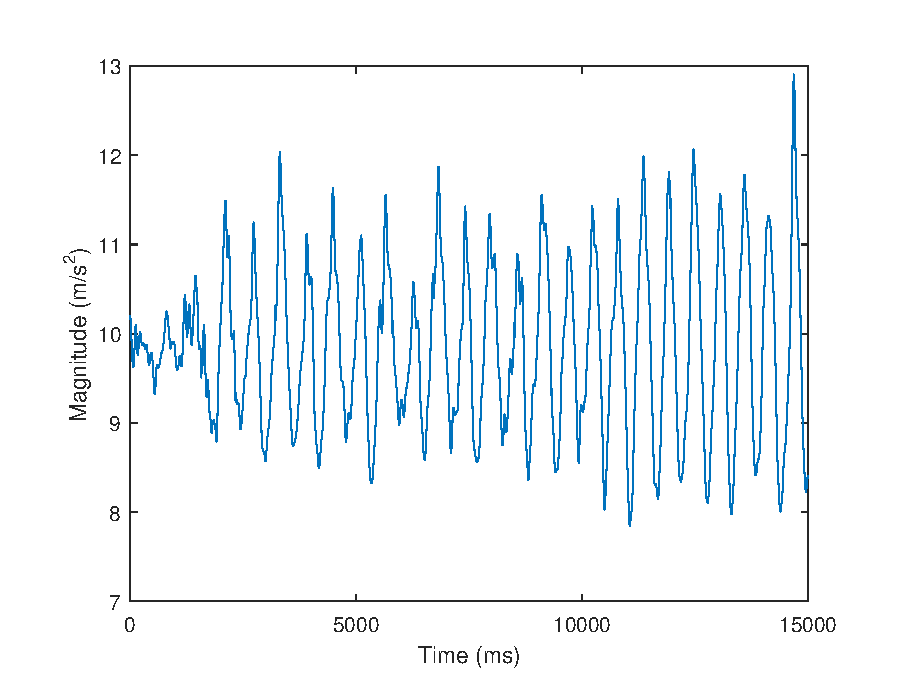
\includegraphics[width=\textwidth]{Images/accel_signal.eps}
            \centering
            \caption{Example of an accelerometer signal over a 15 second period.}
            \label{img_accel_ex}
        \end{figure}

        It is clear that each step will have both a positive and negative peak associated with 2 and 4 respectively. This peak signature will be what the algorithm aims identified in the accelerometer signal. Effectively, the problem boils down to extreme peak detection in a noisy signal. 

        The algorithm is split into 5 stages, each responsible for a particular function in the algorithm. The data will flow from stage to stage much like how a product may move through a pipeline in a factory. All stages have an input queue and output queue, with the exception of the final stage which only has an input queue. At each stage, the data will be adjusted or modified and the algorithm will yield detected steps. A block diagram of this is shown below in Figure \ref{img_sc_block}. Each one of these stages will be described in detail in the following section.

        \begin{figure}[h]
            \includegraphics[width=\textwidth]{Images/step_counter_block.png}
            \centering
            \caption{Block diagram of the step counter algorithm.}
            \label{img_sc_block}
        \end{figure}

    \chapter{Algorithm In-Depth}

        \section{Pre-Processing Stage}

            The Pre-Processing Stage is responsible for two functions:

            \begin{enumerate}
                \item Formatting the data received from the accelerometer into a usable format.
                \item Ensuring a constant sampling frequency by means of linear interpolation.
            \end{enumerate}

            The first step is very straightforward, the magnitude of the signal is computed and the time is zero scaled and put in proper units. The accelerometer data is received in the tri-axial format, but we are interested in the magnitude rather than any single directional component because we do not know the physical orientation of the device. The time should also be scaled appropriately so that the first sample received from the user initiating the algorithm is $t = 0$. The time stamps of the samples are provided in nanoseconds and not given in standard UTC format, but as the time since system boot. The equations for these operations are simple and are as follows:

            \begin{equation}
                m_i = \sqrt{a_{ix}^2 + a_{iy}^2 + a_{iz}^2}
            \end{equation}

            \begin{equation}
                t_{adjusted} = t_i - t_0
            \end{equation}

            The data is then inserted into a simple data structure and is appended to an internal buffer of size 2. When this buffer is full, we will interpolate between these two points. The reason interpolation is needed is that although the developer can specific a desired sample rate in the Android application, there is no guarantee that the accelerometer will be sampled at this rate. An example of this is shown below in Figure \ref{img_sampling_freq} where time between samples is plotted against samples. For the filtering stage, we need to ensure that the data is sampled at a constant rate.



            The algorithm knows what the desired sample rate is, and will interpolate at this value. For example, if the sample rate is set to $f = 100Hz$, then the algorithm will interpolate around $t = 0, 10, 20, 30, ... ms$. Each interpolated point is appended to the end of the stage's output queue. The pseudocode for the linear interpolation is shown below.

            \begin{lstlisting}
time_interval = 10; //ms
count = 0;
while(running):
    if buf is full:
        // Check how many possible interpolated points exist in our interval.
        potential_points = ceil((buf[1].time - buf[0].time) / time_interval);
        for i in range(potential_points):
            if buf[0] <= count * time_interval <= buf[1]:
                // The next interpolated point exists here in this interval
                yield interpolatedPoint(buf[0], buf[1], count * time_interval);
                count++;
        // Get rid of the oldest point
        buf.remove(0)
            \end{lstlisting}

            The maths behind the interpolatedPoint(...) function will be produced below for completeness.

            \begin{equation}
                value = \frac{p_{1,value} - p_{0,value}}{t_{1,value} - t_{0,value}} t_{interpolated} + p_{0,value}
            \end{equation}

            \begin{figure}[h]
                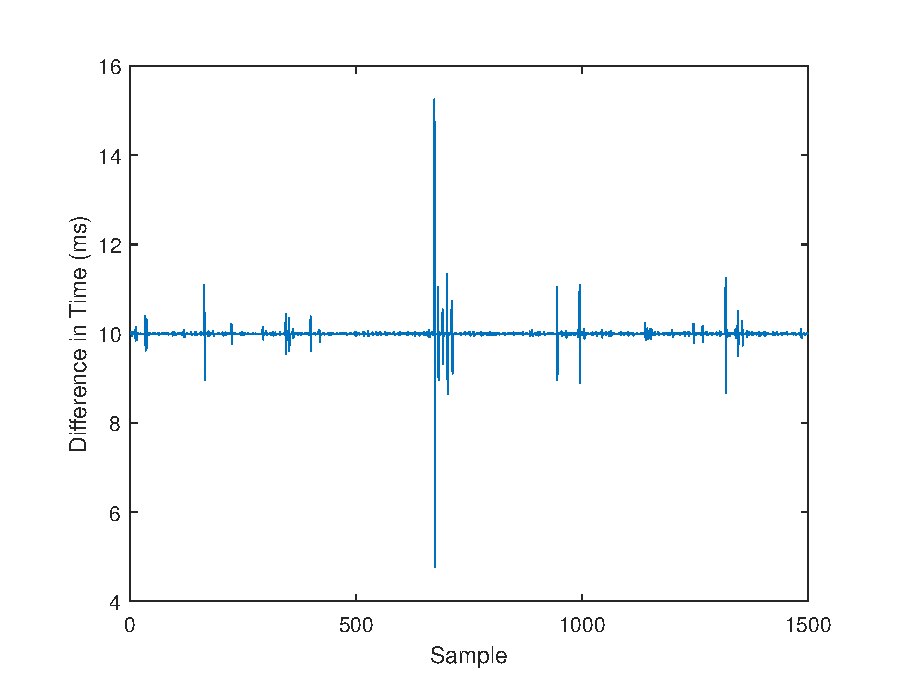
\includegraphics[width=\textwidth]{Images/sampling_freq.eps}
                \centering
                \caption{Time differences between samples for a 100Hz sampled signal.}
                \label{img_sampling_freq}
            \end{figure}

        \section{Filtering Stage}

            The Filtering Stage has one primary function, smooth the signal and remove as much of the high frequency noise from the accelerometer signal.

            The mechanism behind this is a simple FIR, finite impulse response, low-pass digital filter. Ideally, this would be a hard-low pass filter with a frequency response described by [FIG] below. However, this is impossible to achieve due to the infinite impulse response in the time domain (top-hats transform to sinc functions). A few filters were implemented for testing for performance:

            \begin{itemize}
                \item Centered Moving Average - the simplest filter here, the coefficients are simply given by $h_k = \frac{1}{L}$.
                \item Gaussian Window - a slightly more complicated filter, this uses a modified Gaussian function to determine the coefficients.
            \end{itemize}
            [IMG]

        \section{Scoring Stage}

        \section{Detection Stage}

        \section{Post-Processing Stage}

    \chapter{Data Collection Apparatus}

    \chapter{Algorithm Optimization}

    \chapter{Results}

    \chapter{Further Work}